% ============================================================
\chapter{Motivations --- Why Geometry in DL}
\label{ch:motivations}
% ============================================================

Classical neural networks --- MLPs, CNNs, RNNs --- are designed for data
living on regular grids: images on pixels, time series on uniformly spaced
steps. But what do you do when data lives on a graph (social networks,
molecules), on a curved surface (3D models), or on a symmetry group (poses,
rotations)? This is the question that \emph{geometric deep learning}
answers: an architectural revolution, driven by the work of Bronstein,
Bruna, Cohen, and others, that places geometry back at the heart of deep
learning.

% ------------------------------------------------------------
\section{Limitations of Classical Architectures}
% ------------------------------------------------------------

Convolutional neural networks (CNNs) have achieved spectacular success in
computer vision, signal processing, and speech recognition. Their power stems
from a fundamental \textbf{inductive bias}: exploiting the regular grid
structure of data.

\begin{definition}[Inductive bias]
An \textbf{inductive bias} is a set of prior assumptions built into a model's
architecture to guide learning. For a CNN:
\begin{enumerate}
    \item \textbf{Locality}: each neuron sees only a local neighborhood.
    \item \textbf{Weight sharing}: the same filter is applied everywhere.
    \item \textbf{Translation invariance}: pattern detection is independent of position.
\end{enumerate}
\end{definition}

However, many real-world data do \textbf{not} have grid structure:

\begin{example}[Non-Euclidean data]
\begin{enumerate}
    \item A \textbf{molecule} is a graph of atoms connected by chemical bonds.
    \item A \textbf{social network} is a graph of people connected by relationships.
    \item The \textbf{Earth's surface} is a sphere, not a plane.
    \item A \textbf{3D point cloud} from a LiDAR sensor has no canonical ordering.
\end{enumerate}
\end{example}

\begin{warning}[title=\textbf{Why not simply vectorize?}]
One might be tempted to represent a graph by flattening its adjacency matrix
into a vector and using an MLP. This approach fails because:
\begin{itemize}
    \item The representation depends on the \textbf{arbitrary numbering} of nodes.
    \item The number of parameters explodes: $\mathcal{O}(n^2)$ for $n$ nodes.
    \item No \textbf{generalization} to graphs of different sizes.
\end{itemize}
\end{warning}

\section{Geometry as an Organizing Principle}

\subsection{The Erlangen Programme}

In 1872, Felix Klein proposed in his \textit{Erlanger Programm} to classify
geometries by their symmetry groups. This profound idea finds a direct
application in deep learning.

\begin{theorem}[Erlangen Programme --- informal version]
A geometry is entirely determined by its \textbf{transformation group} $G$
and the properties that are \textbf{invariant} under the action of $G$.
\end{theorem}

\begin{example}[Geometries and their groups]
\begin{center}
\begin{tabular}{lll}
\toprule
\textbf{Geometry} & \textbf{Group} & \textbf{Invariants} \\
\midrule
Euclidean & Isometries $\mathrm{E}(n)$ & Distances, angles \\
Affine & Affine transformations & Parallelism, ratios \\
Projective & Projective transformations & Cross-ratio \\
\bottomrule
\end{tabular}
\end{center}
\end{example}

\subsection{From CNNs to GNNs: From Grids to Graphs}

A CNN can be viewed as a special case of a network operating on a regular
graph (the pixel grid), with the translation group $\Z^2$ as its symmetry group.

\begin{keyformulas}[title=\textbf{Discrete convolution on grid vs.\ graph}]
\textbf{Grid convolution}:
\[
    (f * g)(x) = \sum_{y \in \Z^2} f(y)\, g(x - y)
\]
\textbf{Graph convolution} (message passing):
\[
    \mathbf{h}_v^{(\ell+1)} = \phi\!\left(\mathbf{h}_v^{(\ell)},\;
    \bigoplus_{u \in \mathcal{N}(v)} \psi\!\left(\mathbf{h}_v^{(\ell)},
    \mathbf{h}_u^{(\ell)}, \mathbf{e}_{uv}\right)\right)
\]
\end{keyformulas}

\begin{figure}[htbp]
\centering
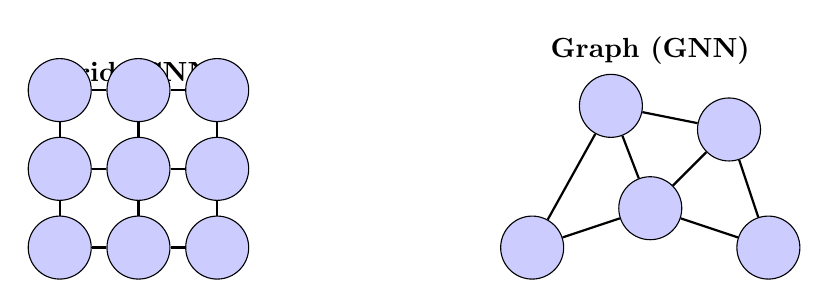
\begin{tikzpicture}[
    node_style/.style={circle, draw, fill=blue!20, minimum size=8mm, inner sep=0pt},
    edge_style/.style={thick, -}
]
% Regular grid 3x3
\begin{scope}[shift={(-4,0)}]
    \node[font=\bfseries] at (1, 2.2) {Grid (CNN)};
    \foreach \i in {0,1,2} {
        \foreach \j in {0,1,2} {
            \node[node_style] (g\i\j) at (\i, \j) {};
        }
    }
    \foreach \i in {0,1,2} {
        \foreach \j [evaluate=\j as \jn using int(\j+1)] in {0,1} {
            \draw[edge_style] (g\i\j) -- (g\i\jn);
        }
    }
    \foreach \j in {0,1,2} {
        \foreach \i [evaluate=\i as \in using int(\i+1)] in {0,1} {
            \draw[edge_style] (g\i\j) -- (g\in\j);
        }
    }
\end{scope}
% Irregular graph
\begin{scope}[shift={(2,0)}]
    \node[font=\bfseries] at (1.5, 2.5) {Graph (GNN)};
    \node[node_style] (a) at (0, 0) {};
    \node[node_style] (b) at (1, 1.8) {};
    \node[node_style] (c) at (2.5, 1.5) {};
    \node[node_style] (d) at (3, 0) {};
    \node[node_style] (e) at (1.5, 0.5) {};
    \draw[edge_style] (a) -- (b);
    \draw[edge_style] (b) -- (c);
    \draw[edge_style] (c) -- (d);
    \draw[edge_style] (a) -- (e);
    \draw[edge_style] (e) -- (b);
    \draw[edge_style] (e) -- (c);
    \draw[edge_style] (e) -- (d);
\end{scope}
\end{tikzpicture}
\caption{From a regular grid (CNN) to an irregular graph (GNN).}
\label{fig:grid_vs_graph}
\end{figure}

\section{The Unifying Framework: Geometric Deep Learning}

\subsection{The Five Gs}

Bronstein et al.\ (2021) proposed a unifying framework organized around five
fundamental domains:

\begin{definition}[GDL Domains]
\begin{enumerate}
    \item \textbf{Grids} ($\Omega = \Z^d$): translation symmetry.
    \item \textbf{Groups} ($\Omega = G$): symmetry by the group itself.
    \item \textbf{Graphs} ($\Omega = (V,E)$): permutation symmetry $S_n$.
    \item \textbf{Geodesics} ($\Omega = \mathcal{M}$): isometry invariance.
    \item \textbf{Gauges} ($\Omega = \mathcal{M}$ with bundle): gauge equivariance.
\end{enumerate}
\end{definition}

\subsection{The General Equivariance Principle}

\begin{theorem}[Equivariance Principle]
Let $\mathfrak{G}$ be a group acting on a signal space
$\mathcal{X}(\Omega)$ via representation $\rho_{\mathcal{X}}$ and on a
target space $\mathcal{Y}$ via $\rho_{\mathcal{Y}}$. A function
$f: \mathcal{X}(\Omega) \to \mathcal{Y}$ is \textbf{equivariant} if:
\[
    f\bigl(\rho_{\mathcal{X}}(g) \cdot x\bigr) = \rho_{\mathcal{Y}}(g) \cdot f(x),
    \quad \forall g \in \mathfrak{G},\; \forall x \in \mathcal{X}(\Omega).
\]
When $\rho_{\mathcal{Y}}$ is the trivial representation, $f$ is
\textbf{invariant}.
\end{theorem}

\begin{intuition}[title=\textbf{Equivariance in pictures}]
Consider image classification:
\begin{itemize}
    \item Convolutional layers are \textbf{equivariant} to translation:
          if the input shifts, the feature maps shift accordingly.
    \item Global pooling produces an \textbf{invariant} output: the result
          does not depend on the object's position.
\end{itemize}
The same principle applies to GNNs: message-passing layers are equivariant
to node permutations, and global readout is invariant.
\end{intuition}

\section{The Importance of Permutation Invariance}

\subsection{Formalization}

For a graph with $n$ nodes, a \textbf{permutation} $\pi \in S_n$ reorders
the nodes. This acts on:
\begin{itemize}
    \item The adjacency matrix: $\mathbf{A} \mapsto \mathbf{P}_\pi \mathbf{A} \mathbf{P}_\pi^\top$
    \item The features: $\mathbf{X} \mapsto \mathbf{P}_\pi \mathbf{X}$
\end{itemize}
where $\mathbf{P}_\pi$ is the permutation matrix associated with $\pi$.

\begin{definition}[Invariant / equivariant functions on graphs]
A graph-level function $f: (\mathbf{A}, \mathbf{X}) \mapsto y$ is
\textbf{permutation invariant} if:
\[
    f(\mathbf{P}_\pi \mathbf{A} \mathbf{P}_\pi^\top, \mathbf{P}_\pi \mathbf{X})
    = f(\mathbf{A}, \mathbf{X}), \quad \forall \pi \in S_n.
\]
A node-level function $f: (\mathbf{A}, \mathbf{X}) \mapsto \mathbf{H}$ is
\textbf{permutation equivariant} if:
\[
    f(\mathbf{P}_\pi \mathbf{A} \mathbf{P}_\pi^\top, \mathbf{P}_\pi \mathbf{X})
    = \mathbf{P}_\pi f(\mathbf{A}, \mathbf{X}), \quad \forall \pi \in S_n.
\]
\end{definition}

\subsection{Deep Sets: The Simplest Case}

\begin{theorem}[Zaheer et al., 2017]
A function $f: 2^{\mathcal{X}} \to \R$ is permutation-invariant and continuous
if and only if it can be written as:
\[
    f(\{x_1, \ldots, x_n\}) = \rho\!\left(\sum_{i=1}^{n} \phi(x_i)\right)
\]
for continuous functions $\phi: \mathcal{X} \to \R^d$ and $\rho: \R^d \to \R$.
\end{theorem}

\begin{codeblock}[title=\textbf{Deep Sets implementation in PyTorch}]
\begin{minted}{python}
import torch
import torch.nn as nn

class DeepSets(nn.Module):
    """Permutation-invariant model for sets."""
    def __init__(self, input_dim, hidden_dim, output_dim):
        super().__init__()
        self.phi = nn.Sequential(
            nn.Linear(input_dim, hidden_dim),
            nn.ReLU(),
            nn.Linear(hidden_dim, hidden_dim),
        )
        self.rho = nn.Sequential(
            nn.Linear(hidden_dim, hidden_dim),
            nn.ReLU(),
            nn.Linear(hidden_dim, output_dim),
        )

    def forward(self, x):
        # x: (batch, n_elements, input_dim)
        h = self.phi(x)           # (batch, n_elements, hidden_dim)
        h = h.sum(dim=1)          # (batch, hidden_dim) -- aggregation
        return self.rho(h)        # (batch, output_dim)

# Test
model = DeepSets(input_dim=3, hidden_dim=64, output_dim=10)
x = torch.randn(8, 20, 3)  # batch=8, 20 points, dim=3
out = model(x)
print(f"Output: {out.shape}")  # (8, 10)

# Verify permutation invariance
perm = torch.randperm(20)
x_perm = x[:, perm, :]
out_perm = model(x_perm)
print(f"Invariant: {torch.allclose(out, out_perm, atol=1e-5)}")
\end{minted}
\end{codeblock}

\section{Motivating Examples}

\subsection{Molecular Property Prediction}

Molecular property prediction is one of the flagship applications of GDL.
A molecule is naturally represented as a graph:
\begin{itemize}
    \item \textbf{Nodes}: atoms, with features (atomic type, charge, etc.).
    \item \textbf{Edges}: chemical bonds, with features (bond order, etc.).
\end{itemize}

\begin{proposition}[Desired properties]
A model for molecular prediction should be:
\begin{enumerate}
    \item \textbf{Permutation invariant} over atoms (no canonical numbering).
    \item \textbf{Rotation and translation invariant} (energy is orientation-independent).
    \item \textbf{Extensive / intensive} depending on the property (energy vs.\ HOMO-LUMO gap).
\end{enumerate}
\end{proposition}

\subsection{Weather on the Sphere}

Weather data naturally lives on the sphere $S^2$. Classical CNNs cannot be
directly applied because:
\begin{itemize}
    \item Planar projections introduce \textbf{distortions} (Mercator, etc.).
    \item The pixel grid is not uniform on the sphere.
    \item Physical symmetries (rotations) are not respected.
\end{itemize}

\begin{remark}[Spherical CNNs]
\textit{Spherical CNNs} (Cohen et al., 2018) define convolutions directly on
$S^2$ using spherical harmonics as a spectral basis, thus respecting
$\mathrm{SO}(3)$ equivariance.
\end{remark}

\subsection{Particle Dynamics}

Simulation of particle systems (fluids, granular materials) benefits from GDL
because:
\begin{itemize}
    \item Particles form an unordered set.
    \item Physical laws are equivariant under $\mathrm{SE}(3)$.
    \item Interactions are local (neighborhood graph).
\end{itemize}

\section{Panorama of Geometric Architectures}

\begin{figure}[htbp]
\centering
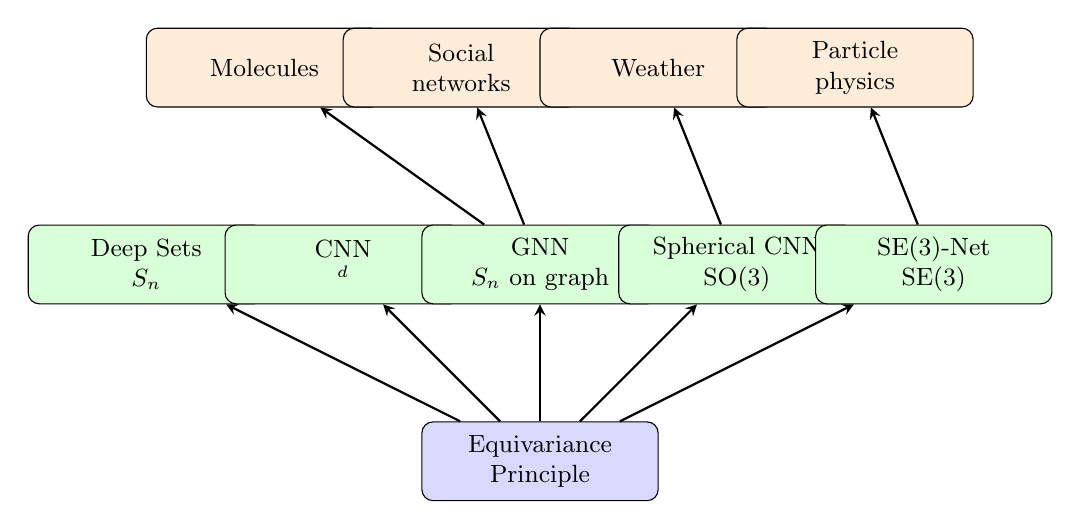
\begin{tikzpicture}[
    box/.style={rectangle, draw, rounded corners, fill=#1!15,
                minimum width=3cm, minimum height=1cm, align=center,
                font=\small},
    arr/.style={->, thick, >=stealth}
]
\node[box=blue] (base) at (0, 0) {Equivariance\\Principle};
\node[box=green] (ds) at (-5, 2.5) {Deep Sets\\$S_n$};
\node[box=green] (cnn) at (-2.5, 2.5) {CNN\\$\Z^d$};
\node[box=green] (gnn) at (0, 2.5) {GNN\\$S_n$ on graph};
\node[box=green] (scnn) at (2.5, 2.5) {Spherical CNN\\$\mathrm{SO}(3)$};
\node[box=green] (se3) at (5, 2.5) {SE(3)-Net\\$\mathrm{SE}(3)$};

\draw[arr] (base) -- (ds);
\draw[arr] (base) -- (cnn);
\draw[arr] (base) -- (gnn);
\draw[arr] (base) -- (scnn);
\draw[arr] (base) -- (se3);

\node[box=orange] (mol) at (-3.5, 5) {Molecules};
\node[box=orange] (soc) at (-1, 5) {Social\\networks};
\node[box=orange] (met) at (1.5, 5) {Weather};
\node[box=orange] (phys) at (4, 5) {Particle\\physics};

\draw[arr] (gnn) -- (mol);
\draw[arr] (gnn) -- (soc);
\draw[arr] (scnn) -- (met);
\draw[arr] (se3) -- (phys);
\end{tikzpicture}
\caption{Panorama of geometric architectures and their applications.}
\end{figure}

\section{Why Symmetries Improve Learning}

Exploiting symmetries improves learning in three complementary ways:

\begin{theorem}[Benefits of equivariance]
Let $\mathfrak{G}$ be the symmetry group of a problem. An equivariant model
benefits from:
\begin{enumerate}
    \item \textbf{Sample complexity reduction}: the number of required examples
          is reduced by a factor of $\abs{\mathfrak{G}}$ (or the group dimension
          for continuous groups).
    \item \textbf{Improved generalization}: generalization to all transformations
          in $\mathfrak{G}$ is guaranteed ``for free.''
    \item \textbf{Weight sharing}: parameter count is reduced, avoiding overfitting.
\end{enumerate}
\end{theorem}

\begin{proposition}[Generalization bound]
For a model parameterized by $\theta \in \Theta$, the Rademacher complexity of
the equivariant function class $\mathcal{F}_{\text{equiv}}$ satisfies:
\[
    \mathfrak{R}_n(\mathcal{F}_{\text{equiv}}) \leq
    \frac{\mathfrak{R}_n(\mathcal{F})}{\sqrt{\abs{\mathfrak{G}}}}
\]
where $\mathcal{F}$ is the unconstrained class.
\end{proposition}

\section{From Theory to Practice}

\begin{codeblock}[title=\textbf{First GNN with PyTorch Geometric}]
\begin{minted}{python}
import torch
import torch.nn.functional as F
from torch_geometric.nn import GCNConv, global_mean_pool
from torch_geometric.datasets import TUDataset
from torch_geometric.loader import DataLoader

class SimpleGNN(torch.nn.Module):
    def __init__(self, num_features, num_classes):
        super().__init__()
        self.conv1 = GCNConv(num_features, 64)
        self.conv2 = GCNConv(64, 64)
        self.lin = torch.nn.Linear(64, num_classes)

    def forward(self, data):
        x, edge_index, batch = data.x, data.edge_index, data.batch
        # Permutation-equivariant layers
        x = F.relu(self.conv1(x, edge_index))
        x = F.relu(self.conv2(x, edge_index))
        # Permutation-invariant readout
        x = global_mean_pool(x, batch)
        return self.lin(x)

# Load a graph classification dataset
dataset = TUDataset(root='/tmp/MUTAG', name='MUTAG')
loader = DataLoader(dataset, batch_size=32, shuffle=True)

model = SimpleGNN(dataset.num_features, dataset.num_classes)
optimizer = torch.optim.Adam(model.parameters(), lr=0.01)

# Training loop
for epoch in range(50):
    total_loss = 0
    for data in loader:
        optimizer.zero_grad()
        out = model(data)
        loss = F.cross_entropy(out, data.y)
        loss.backward()
        optimizer.step()
        total_loss += loss.item()
    if (epoch + 1) % 10 == 0:
        print(f"Epoch {epoch+1}, Loss: {total_loss/len(loader):.4f}")
\end{minted}
\end{codeblock}

\section{Course Outline and Dependencies}

\begin{figure}[htbp]
\centering
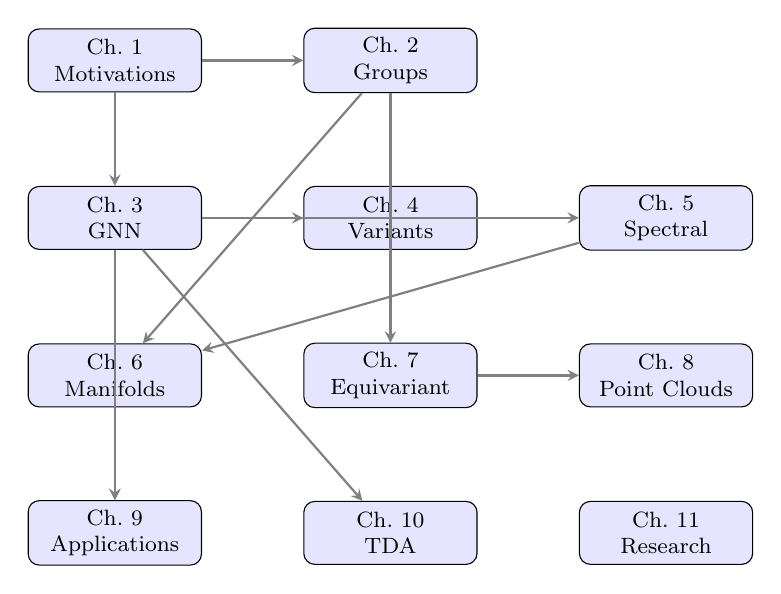
\begin{tikzpicture}[
    ch/.style={rectangle, draw, rounded corners, fill=blue!10,
               minimum width=2.2cm, minimum height=0.8cm,
               align=center, font=\footnotesize},
    dep/.style={->, thick, >=stealth, gray}
]
\node[ch] (c1) at (0, 0) {Ch.~1\\Motivations};
\node[ch] (c2) at (3.5, 0) {Ch.~2\\Groups};
\node[ch] (c3) at (0, -2) {Ch.~3\\GNN};
\node[ch] (c4) at (3.5, -2) {Ch.~4\\Variants};
\node[ch] (c5) at (7, -2) {Ch.~5\\Spectral};
\node[ch] (c6) at (0, -4) {Ch.~6\\Manifolds};
\node[ch] (c7) at (3.5, -4) {Ch.~7\\Equivariant};
\node[ch] (c8) at (7, -4) {Ch.~8\\Point Clouds};
\node[ch] (c9) at (0, -6) {Ch.~9\\Applications};
\node[ch] (c10) at (3.5, -6) {Ch.~10\\TDA};
\node[ch] (c11) at (7, -6) {Ch.~11\\Research};

\draw[dep] (c1) -- (c2);
\draw[dep] (c1) -- (c3);
\draw[dep] (c2) -- (c7);
\draw[dep] (c3) -- (c4);
\draw[dep] (c3) -- (c5);
\draw[dep] (c2) -- (c6);
\draw[dep] (c5) -- (c6);
\draw[dep] (c7) -- (c8);
\draw[dep] (c3) -- (c9);
\draw[dep] (c6) -- (c9);
\draw[dep] (c3) -- (c10);
\end{tikzpicture}
\caption{Dependency graph between chapters.}
\end{figure}

\section*{Exercises}

\begin{exercise}[Invariance vs.\ equivariance]
Let $f: \R^{n \times d} \to \R^{n \times d'}$ be defined by
$f(\mathbf{X}) = \sigma(\mathbf{X}\mathbf{W})$ where $\mathbf{W} \in \R^{d \times d'}$.
\begin{enumerate}
    \item Show that $f$ is equivariant to permutation of the rows of $\mathbf{X}$.
    \item Propose a modification of $f$ to obtain an invariant function
          $g: \R^{n \times d} \to \R^{d'}$.
    \item Implement both functions in PyTorch and verify experimentally.
\end{enumerate}
\end{exercise}

\begin{exercise}[Limitations of vectorization]
Consider a random graph $G \sim \mathrm{Erd\H{o}s\text{-}R\acute{e}nyi}(n, p)$.
\begin{enumerate}
    \item How many different matrix representations $\mathbf{A}$ correspond to
          the same (isomorphic) graph?
    \item Deduce why an MLP applied to $\mathrm{vec}(\mathbf{A})$ has exponential
          sample complexity.
    \item Show that a GNN avoids this problem by construction.
\end{enumerate}
\end{exercise}

\begin{exercise}[Deep Sets for symmetric function approximation]
Implement a Deep Sets model to approximate the function
$f(\{x_1, \ldots, x_n\}) = \max_i x_i - \min_i x_i$ (the range of a set).
\begin{enumerate}
    \item Train the model on sets of variable size $n \in [5, 50]$.
    \item Evaluate generalization to $n = 100$.
    \item Compare with a $\max$ aggregation instead of sum.
\end{enumerate}
\end{exercise}
